\documentclass[main]{subfiles}
\begin{document}
%@@@@@@@@@@@@@@@@@@@@@@@@@@@@@@
% summarizes lecture 4
% author: Joachim Ott

\section{Current Mirror}
% Joachim
The current mirror circuit is built by connection the gate of a diode-connected transistor to the gate of another transistor.
Both transistors have a fixed source voltage, are in saturation, and act as a current source.


\begin{figure}[htbp]
  \centering
  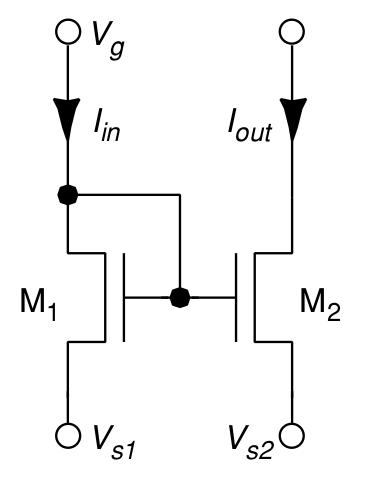
\includegraphics[scale=1]{figs/current_mirror_vlsi.png}
  \caption{nFET Current Mirror \cite{book:VLSI}}
  \label{fig:nFET_Current_Mirror}
\end{figure}\bigskip

\begin{itemize}
\item M1: Diode connected transistor
\item Input current $I_{in}$ sets common gate voltage $V_g$, hence also sets $I_{out}$
\end{itemize}

\subsection{Scaling of $I_{in}$ vs $I_{out}$}
\begin{itemize}
\item By choosing different source potentials $V_{s1}$ and $V_{s1}$
\subitem Leads to exponential scaling: $I_{out}=e^{V_{s1}-V_{s2}/U_T} \cdot I_{in}$
\item By choosing different transistor sizes
\subitem The current scales linearly with transistor size difference 
\subitem Important: Fixed transistor width vs. length ratio
\end{itemize}

\subsection{Above Threshold Operation}
Input vs. output currents depends mainly on drain voltage of $M_1$ and $M_2$, because of larger Early effect. The dependence on the source voltage is much weaker.\\
With bidirectional input, the current mirror can be used as half wave rectifier, because the input transistor has high impedance in the opposite direction.

\begin{figure}[htbp]
  \centering
  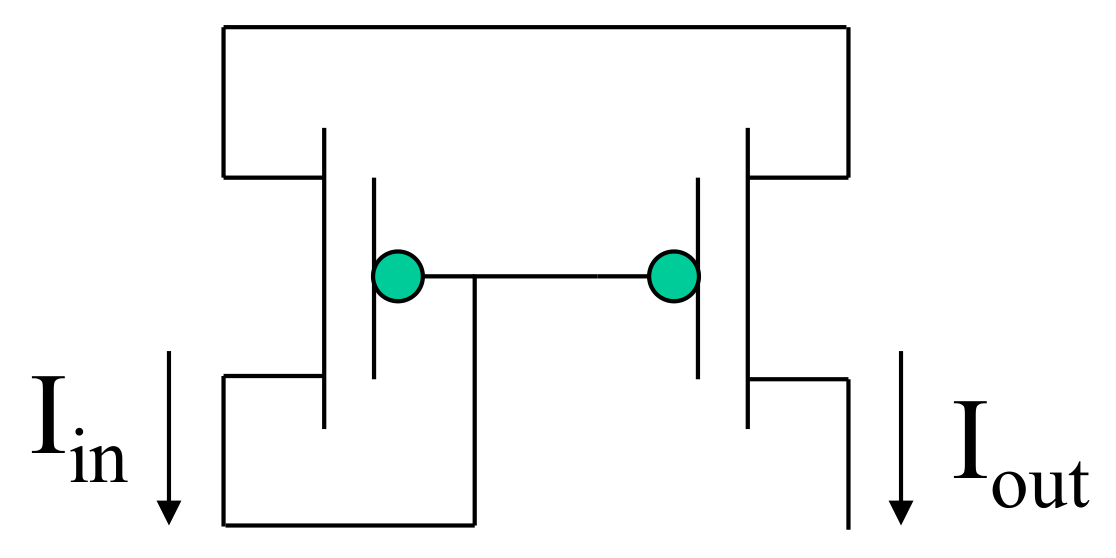
\includegraphics[scale=0.5]{figs/current_mirror_pfet.png}
  \caption{pFET Current Mirror \cite{lec4}}
  \label{fig:pFET_Current_Mirror}
\end{figure}\bigskip
\end{document}